% Self-contained manuscript: bibliography and vector diagrams are embedded.
% Compile with pdfLaTeX twice, or Tectonic. No shell escape or external assets.
% Template: mystyle.cls from arXiv:2601.14004v4 (2026-04-14).
% Original class declares CC BY-SA 4.0 and RAIL/DeepMind template provenance.
% Original notice is preserved below. Adaptation: remove unrelated dormant author text.
% Manuscript framework is independent of the reference paper's content framework.
% Standalone distribution: the embedded class is written locally on compilation.
\begin{filecontents*}{mystyle.cls}
%%%%%%%%%
%
% Style file used by UC Berkeley RAIL folks.
% This is an edited version of the Google DeepMind tech report template, used under CC Licence, obtained from tex sources of Google DeepMind arxiv papers. There are several changes including font sizes, abstract formatting, title formatting, figure formatting, colors, and math fonts which are allowed per the license.
% 
%
% Use it in the following way, with the full set of option possible:
% \documentclass[11pt, a4paper, twocolumn, logo, copyright, nonumbering, 
% internal]{berkeley} 
%
% Options:
%    - 11pt: Sets the normal font size of the text. Can be only 10, 11, 12pt.
%    - a4paper: Paper size. Usually would not adjust.
%    - twocolumn: Makes the paper into two column mode; single column by default.
%    - logo: Adds the BAIR logo to the top left. No logo included if left out.
%    - copyright: Add a copyright statement to the first page of the paper in the left footnote
%    - nonumbering: Uses unnumbered sections.
%    - internal: for internal only docs that should not be shared externally. 
%           Can only use techreportnumber with this option.
%
% Date of Paper
%   The report is by default given the curren date in the top right. If you want to fix the 
%   date: add the date to your preamble with your own date as follows:
%   \renewcommand{\today}{1 January 2000}
%
% Confidentiality
%   Change the confidentiality statement for internal docs by adding this in the preable 
%   \renewcommand{\internal}{Confidential.}
%   
% ----------------
% Licence: This template is released under the Creative Commons licence 
% Attribution-ShareAlike 4.0 International (CC BY-SA 4.0)
%
%
% Known issues:
%   - Package todonotes does not work in the abstract
%
% Version history: 
% v0.1 - Jan 2024: Obtained from arxiv papers
% v0.2 - Feb 2024: revised some details
% %%%%%%%%%%%%%%%


\NeedsTeXFormat{LaTeX2e}

% Palatino font %%%%---- to switch to computer modern font, comment next three lines, and line 126
\RequirePackage{tgpagella} % text only
\RequirePackage{mathpazo}  % math & text
\RequirePackage{inconsolata} % for tt font



%%======== Pckage options and base class ========
\RequirePackage{tcolorbox}
\RequirePackage{xifthen}
\newboolean{nonumbering}
\newboolean{logo}
\newboolean{address}
\newboolean{copyright}
\newboolean{internal}
\DeclareOption{nonumbering}{\setboolean{nonumbering}{true}}
\DeclareOption{logo}{\setboolean{logo}{true}}
\DeclareOption{address}{\setboolean{address}{true}}
\DeclareOption{copyright}{\setboolean{copyright}{true}}
\DeclareOption{internal}{\setboolean{internal}{true}}
\DeclareOption*{\PassOptionsToClass{\CurrentOption}{extarticle}}
\ProcessOptions
\LoadClass{extarticle}

%%======== Packages Required ========
% Fonts and language
\AtEndOfClass{\RequirePackage{microtype}}
\RequirePackage[utf8]{inputenc}
\RequirePackage[english]{babel}
\RequirePackage{amsthm, amsmath, amsfonts, amssymb}
\RequirePackage{cmap}
\RequirePackage[T1]{fontenc}
\RequirePackage{url}
\RequirePackage{pifont}
\RequirePackage{textcomp} % For copyright symbol styling
\RequirePackage[overload]{textcase}
%\RequirePackage{balance}
%% *Graphics, tables and other formatting
\RequirePackage{graphicx}
\RequirePackage{colortbl}

\RequirePackage{booktabs}
\RequirePackage{changepage}
\RequirePackage{enumitem} % For reducing bullet list item separation
\RequirePackage{tabularx}
\RequirePackage{datetime}
% Headers and footers
\RequirePackage{fancyhdr}  % custom headers/footers
\RequirePackage{lastpage}  % Number of pages in the document
% Lists and their spacing
\RequirePackage{enumitem}
\setlist[itemize]{noitemsep}
\setlist[enumerate]{noitemsep}
% % Title, Abstract, Bibliography
\RequirePackage[explicit]{titlesec}
\RequirePackage{bibentry}
\RequirePackage{mdframed}
\RequirePackage{caption}
\RequirePackage{needspace}

% \RequirePackage[svgnames]{xcolor}
\definecolor{TinaCrimson}{HTML}{DC143C} % Renamed from Crimson
% \RequirePackage[dvipsnames]{xcolor}
% \definecolor{Crimson}{HTML}{990000}

\definecolor{CalGoldHex}{HTML}{fff7e8}
% \definecolor{CalGoldHex}{HTML}{FFF5E1}
\definecolor{IronGrey}{HTML}{6D6E71}
\definecolor{LARGBlue}{HTML}{4381BA}

\RequirePackage[colorlinks=true, allcolors=LARGBlue]{hyperref}

%%======== Can use any of these fonts ========
% \RequirePackage{charter}
% \RequirePackage[scaled]{helvet}
% \RequirePackage{bookman}
% \RequirePackage{times}
% \RequirePackage[default]{opensans} %fosfamily
%\usepackage{antpolt}
% Math fonts
% \RequirePackage{mathpazo} % Palatino
%\usepackage{euler} % for math fints

% Use Bitstream Charter as the main font. Does not include a typewriter font.
\RequirePackage[type1]{XCharter} %%%%---- to switch to computer modern font, comment this line, and lines 47-49
% \RequirePackage[xcharter,bigdelims,vvarbb]{newtxmath}
% \RequirePackage{libertine}
% \RequirePackage{libertinust1math}
% \RequirePackage[p]{zlmtt} % for teletype, lmodern's typewriter font


% Use the typewriter font from lmodern, scaled up to match Charter's xheight.
% You may wish to add the "p" option to use the proportional font instead of
% the monospaced one, which might look nicer in cases where you do not need
% aligned columns
\RequirePackage[scaled=1.1]{zlmtt}
% \RequirePackage{libertine}
% \RequirePackage{libertinust1math}

%%======== Margins and column spacing ========
\RequirePackage[left=1.9cm,%
right=1.9cm,%
top=3cm,%
bottom=2.5cm,%
headheight=40pt,%
headsep=20pt,%
%showframe, % for testing
letterpaper]{geometry}%
\setlength{\columnsep}{15pt} % Distance between the two columns of text
%\setlength{\parindent}{0pt}
\setlength{\parskip}{0.5\baselineskip}

%% *Custom font sizes and styles
\newcommand{\watermarkfont}{\color{black50}\normalfont\fontsize{10}{12}\selectfont}
\newcommand{\headerfont}{\color{LARGBlue}\normalfont\sffamily\fontsize{8}{10}\selectfont}
% \newcommand{\titlefont}{\color{LARGBlue}\normalfont\bfseries\fontsize{21}{23}\selectfont} %%%%---- title font/color
\newcommand{\titlefont}{\centering\color{LARGBlue}\normalfont\fontsize{21}{23}\selectfont} %%%%---- title font/color
\newcommand{\datesfont}{\normalfont\sffamily\itshape\fontsize{8}{10}\selectfont}
\newcommand\urlheaderfont{\color{LARGBlue}\fontsize{8}{10}\selectfont}
\newcommand{\absfont}{\linespread{1.1}\fontsize{10}{12}\color{black}\selectfont}
\newcommand{\keywordstitlefont}{\bfseries\linespread{1.2}\fontsize{8}{10}\selectfont}
\newcommand{\keywordsfont}{\itshape\linespread{1.2}\fontsize{11}{12}\selectfont}
\newcommand{\copyrightfont}{\normalfont\fontsize{7}{9}\selectfont}
\newcommand{\footerfont}{\color{black}\normalfont\fontsize{8}{10}\selectfont}
\newcommand{\subjectfont}{\color{white}\bfseries\fontsize{10}{12}\selectfont}
\newcommand{\headingfont}{\color{LARGBlue}\bfseries\fontsize{13}{14}\selectfont}

\newcommand{\keywords}[1]{\def\@keywords{#1}}
\newtoks\correspondingauthor
\newtoks\paperurl
\newtoks\reportnumber

% Dates and Times for footer
%\newdateformat{monthyeardate}{\THEDAY{ }\monthname[\THEMONTH] \THEYEAR}
% ISO-8601 date format
\newdateformat{monthyeardate}{\THEYEAR-\THEMONTH-\THEDAY}
\setcounter{secnumdepth}{3}
\ifthenelse{\boolean{nonumbering}}{\setcounter{secnumdepth}{0}}{}

%%========  Author and affiliation ========
\RequirePackage{authblk}
\setcounter{Maxaffil}{0}
\setlength{\affilsep}{0.2em}
\renewcommand\Authfont{\centering\normalfont\bfseries\fontsize{10}{14}\selectfont}
\renewcommand\Affilfont{\centering\normalfont\fontsize{10}{20}\selectfont}
\makeatletter
\renewcommand\AB@affilsepx{, \protect\Affilfont}
\makeatother
\renewcommand\Authands{, and }

\newcommand{\internalonly}{}
\newcommand{\copyrightext}{\footerfont \textcopyright\, \the\year{} }


%%======== Header and Footer Content ========
%
% Header and Footer for the first page
\pagestyle{fancy}   % Enables the custom headers/footers
\fancypagestyle{firststyle}{
	\fancyhead[L]{
		\ifthenelse{\boolean{logo}}{
			\includegraphics[width=90pt]{assets/berkeley_logo}
	 }{}
}
\fancyhead[R]{
	\ifdefined\paperurl
	\if\relax\the\paperurl\relax \else
		\href{\the\paperurl}{\urlheaderfont \itshape \the\paperurl}\\ \fi
	\else \fi
	{}
}
\fancyhead[C]{}
\renewcommand{\headrulewidth}{0pt}
\renewcommand{\footrulewidth}{1pt}
%
\fancyfoot[L]{
	\ifdefined\correspondingauthor
	\if\relax\the\correspondingauthor\relax
	\else \footerfont\itshape  {Corresponding author(s): \the\correspondingauthor \\} \fi
	\else \fi
    \ifthenelse{\boolean{internal}}{\footerfont \internalonly \\}{\footerfont\bfseries\relax}
	\ifthenelse{\boolean{address}}{
		\itshape\footerfont UC Berkeley, Berkeley, California \\}{}
	\ifthenelse{\boolean{copyright}}{\copyrightext}{}
}
\fancyfoot[R]{
	\ifthenelse{\boolean{internal}}{
	\ifdefined\reportnumber
	\if\relax\the\reportnumber\relax
	\else \footerfont\itshape  {\footerfont \bfseries \the\reportnumber} \fi
	\else \fi
	}{\footerfont\bfseries\relax}
}
\fancyfoot[C]{\footerfont\bfseries\relax}}



% Header and Footer for pages from 2 onwards
\renewcommand{\footrulewidth}{0pt}
\fancyhead[L,R]{}
\makeatletter
\newcommand\runningtitle[1]{\renewcommand\@runningtitle{#1}}
\newcommand\@runningtitle{}
\fancyhead[C]{\footerfont \@runningtitle} %%%%---- Running title
\makeatother
\fancyfoot[C]{}
\fancyfoot[L]{
	\ifthenelse{\boolean{internal}}{\footerfont \internalonly\newline
		\ifdefined\reportnumber
		\if\relax\the\reportnumber\relax
		\else \footerfont {} \fi
		\else \fi}{\footerfont\bfseries\relax}
}
\fancyfoot[R]{\footerfont \thepage}

% Header and footer rules (coloured).
\renewcommand{\headrulewidth}{1pt}
% \renewcommand{\footrulewidth}{1pt}
\let\DefaultHeadRule\headrule
\let\DefaultFootRule\footrule
\renewcommand{\headrule}{\color{black}\DefaultHeadRule}
\renewcommand{\footrule}{\textcolor{black}{\DefaultFootRule}}
\definecolor{LightYellow}{HTML}{FFFCEF}    % 浅黄色
\definecolor{DarkYellow}{HTML}{F2E0BD}     % 深黄色/金色
\definecolor{LightBlue}{HTML}{F3F9FE}    % 浅黄色
\definecolor{DarkBlue}{HTML}{326A9D}     % 深黄色/金色
\tcbset{
    titlebox/.style={
        colback=LightBlue,           % 浅黄色背景
        colframe=DarkBlue,    % 深黄色边框
        boxrule=2pt,                 % 边框粗细
        arc=0mm,                     % 微微的圆角
        % 只显示上下边框的技巧
        leftrule=0pt,
        rightrule=0pt,
        left=5mm,
        right=5mm,
        top=5mm,
        bottom=5mm
    }
}

\renewenvironment{abstract}
{\par\noindent\\  \ignorespaces}
{\par\bigskip}


%%========  Bibliography using bibtex ========


\addto{\captionsenglish}{\renewcommand{\refname}{References}}
\newcommand{\citeas}[1]{\Needspace*{8\baselineskip}\noindent\bibentry{#1}}
% Uncomment the next line if you want the  numbered refs to be "1." instead of "[1]".
%\makeatletter \renewcommand\@biblabel[1]{#1.} \makeatother

%%======== Abstract and section formatting ========


\def\xabstract{abstract}
\long\def\abstract#1\end#2{\def\two{#2}\ifx\two\xabstract
	\long\gdef\theabstract{\ignorespaces#1}
	\def\go{\end{abstract}}\else
\typeout{^^J^^J PLEASE DO NOT USE ANY \string\begin\space \string\end^^J
	COMMANDS WITHIN ABSTRACT^^J^^J}#1\end{#2}
\gdef\theabstract{\vskip12pt BADLY FORMED ABSTRACT: PLEASE DO
NOT USE {\tt\string\begin...\string\end} COMMANDS WITHIN
THE ABSTRACT\vskip12pt}\let\go\relax\fi
\go}

% Define an environment with abstract content and styling
\makeatletter
\newcommand{\abscontent}{
	\noindent
	\parbox{\dimexpr\linewidth}{\absfont \theabstract}
	\@ifundefined{@keywords}{}{
		\vskip1em \noindent \keywordsfont  Keywords: \@keywords}
}

\newcommand{\HorRule}{\color{black}\rule{\textwidth}{1pt}} %

\if@twocolumn%
\renewcommand{\maketitle}{
	\twocolumn[
	\begin{adjustwidth}{0pt}{24pt}
		\begin{center}
			{
                    % % \vskip-0.5cm
                    % \HorRule
                    \vskip5pt
				{\raggedright \titlefont
				\@title\par}%
				\vskip11pt
				{\raggedright \@author\par}
				\vskip-5pt%
                    \HorRule
                    \vskip10pt%
			}%
		\end{center}
	\end{adjustwidth}
		\abscontent
	\vskip20pt%
	]
	% \thispagestyle{firststyle}
}%
\else% \@twocolumnfalse
\renewcommand{\maketitle}
{
\vphantom{a}
\vspace{-15mm}
\begin{tcolorbox}[titlebox]
\bgroup\setlength{\parindent}{0pt}
	\begin{adjustwidth}{0pt}{24pt}
		\begin{center}
			{
                    \centering
                    % \vskip-100pt
                    % \HorRule
                    \vskip5pt
				{\raggedright \titlefont \textbf{\@title}\vspace{5mm}\par}% %%%%---- title definition
				\vskip11pt
				{\raggedright \@author\par}
                    \vskip15pt%
			}%
		\end{center}
	\end{adjustwidth}
	\egroup
	{%
		{\abscontent}
	}%
	% \thispagestyle{firststyle}
 \end{tcolorbox}
}%
\fi
\makeatother

\titleformat{\section}
{\large\bfseries\headingfont}
{\thesection.}
{0.5em}
%{\MakeUppercase{#1}}[]
{#1}
[]

\titleformat{name=\section,numberless}
{\large\bfseries\headingfont}
{}
{0em}
%{\MakeUppercase{#1}}[]
{#1}
[]
\titleformat{\subsection}
{\bfseries}
{\thesubsection.}
{0.5em}
{#1}
[]
\titleformat{\subsubsection}% [runin] If want to have inline for the subsubsect
{\bfseries\itshape}
{\thesubsubsection.}
{0.5em}
{#1}
[]


\titlespacing*{\section}{0pc}{3ex plus4pt minus3pt}{5pt}
%\titlespacing*{\section}{0pc}{1ex }{\baselineskip}
\titlespacing*{\subsection}{0pc}{2.5ex plus3pt minus2pt}{2pt}
\titlespacing*{\subsubsection}{0pc}{2ex plus2.5pt minus1.5pt}{2pt}
%\titlespacing*{\paragraph}{0pc}{2ex plus2pt minus1pt}{0pt}

%%======== Captions in tables and figures ========
\DeclareCaptionLabelSeparator{pipe}{:~}% or $\vert$
\captionsetup{labelfont={}, %{bf,sf},%
labelsep=space,%
figurename=\textbf{Figure},%
labelsep=pipe,
singlelinecheck=off,%
%justification=centering
}


\end{filecontents*}
\documentclass[11pt,letterpaper]{mystyle}
\usepackage[T1]{fontenc}
\usepackage[utf8]{inputenc}
\usepackage{microtype}
\geometry{margin=1in}
\usepackage{amsmath,amssymb,mathtools}
\usepackage{booktabs,longtable,array,tabularx}
\usepackage{xcolor}
\usepackage{enumitem}
\usepackage{graphicx}
\usepackage{flafter}
\usepackage[section]{placeins}
\usepackage{tikz}
\usetikzlibrary{arrows.meta,positioning,fit}
\captionsetup{font=small,labelfont=bf}
\usepackage{fancyhdr}
\usepackage[numbers,sort&compress]{natbib}
\definecolor{darkblue}{rgb}{0,0.40,0.75}
\hypersetup{pdfauthor={Zunhai Su},pdftitle={Training--Rollout Mismatch in Low-Precision LLM Reinforcement Learning: A Survey},colorlinks=true,linkcolor=darkblue,citecolor=darkblue,urlcolor=darkblue,breaklinks=true}
\usepackage{url}
\definecolor{navy}{HTML}{18344F}
\definecolor{bluewash}{HTML}{EDF3F9}
\definecolor{tealwash}{HTML}{EAF5F2}
\definecolor{redwash}{HTML}{FBECE8}
\definecolor{redwarn}{HTML}{A74835}
% Compact manuscript-level adaptation of the supplied title panel.
\renewcommand\Affilfont{\centering\normalfont\fontsize{10}{12}\selectfont}
\makeatletter
\renewcommand{\maketitle}{%
\begin{tcolorbox}[titlebox,top=2mm,bottom=2mm,left=4mm,right=4mm]
\setlength{\parskip}{3pt}
{\centering\color{LARGBlue}\bfseries\fontsize{18.5}{21}\selectfont\@title\par}
\vspace{2mm}
{\centering\@author\par}
\vspace{2mm}
\noindent\parbox{\linewidth}{\absfont\theabstract}
\end{tcolorbox}\vspace{-1mm}}
\makeatother
\newcolumntype{Y}{>{\raggedright\arraybackslash}X}
\newcolumntype{P}[1]{>{\raggedright\arraybackslash}p{#1}}
\newcommand{\E}{\mathbb{E}}
\newcommand{\KL}{D_{\mathrm{KL}}}
\newcommand{\sg}{\operatorname{sg}}
\newcommand{\clip}{\operatorname{clip}}
\newcommand{\takeaway}[1]{\par\medskip\noindent\colorbox{bluewash}{\parbox{\dimexpr\linewidth-2\fboxsep\relax}{\textbf{Synthesis.} #1}}\par\medskip}
\newcommand{\discussion}[2]{\par\medskip\noindent\fcolorbox{navy}{tealwash}{\parbox{\dimexpr\linewidth-2\fboxsep-2\fboxrule\relax}{\textbf{#1}\par\smallskip #2}}\par\medskip}
\setlist{itemsep=2pt,topsep=4pt}
\setlength{\emergencystretch}{2em}
\clubpenalty=10000
\widowpenalty=10000
\runningtitle{Training--Rollout Mismatch in Low-Precision LLM Reinforcement Learning}
\title{\textbf{Training--Rollout Mismatch in Low-Precision LLM Reinforcement Learning: A Survey}}
\setcounter{Maxaffil}{1}
\author{Zunhai Su}
\affil{The University of Hong Kong}
\date{Literature snapshot: October 19, 2026}
\begin{document}
\begin{abstract}
\textbf{Abstract:} 
Low-precision rollout generation can reduce execution cost while changing the numerical policy that supplies reinforcement-learning data. The resulting training--rollout mismatch links numerical approximation to gradient estimation, policy updates, and the trajectories encountered later in training. This survey reviews twenty focal studies through a common account of that feedback. We separate same-snapshot execution differences from policy staleness and decoding transformations, and distinguish conditional correction from response-level change of measure. A component-level taxonomy organizes numerical alignment and fidelity control alongside estimator correction, policy-update control, and schedule adaptation. We then compare the mechanisms these interventions target, the information they require, and the evidence supporting their learning and efficiency claims. Three findings recur: correction must be assessed over the learning trajectory; numerical coupling is meaningful at a specified execution interface; and the signed updates retained by an objective can matter more than an aggregate discrepancy statistic. Together, these findings position numerical fidelity and learning correction as complementary design resources. The survey closes with priorities in predictive diagnosis, method composition, stateful collection, and transferable evidence, supported by a versioned bibliography and an evolving public resource collection.
\par\medskip
\noindent\textbf{Keywords:} quantized rollout; low-precision reinforcement learning; training--inference mismatch; importance sampling; quantization-aware training.
\par\medskip\textbf{Literature snapshot:} October 19, 2026.
\par\medskip\noindent\textbf{Survey resources:} \url{https://github.com/ZunhaiSu/awesome-low-precision-rl}
\par\smallskip\noindent\textit{Living survey, under active development. Suggestions, corrections, and research collaborations are welcome via \href{https://github.com/ZunhaiSu/awesome-low-precision-rl/issues}{GitHub Issues}.}
\end{abstract}
\maketitle\thispagestyle{empty}
% The introduction continues on page one; the full contents follows Section 1.

\section{Introduction and Scope}\label{sec:intro}
\subsection{Why Low-Precision Rollouts Complicate Policy Optimization}
In language-model reinforcement learning, the sampler is part of the learning algorithm: it determines the responses, rewards, and histories from which the next policy is learned. A numerical approximation therefore changes both an execution path and a source of training data. Its consequences can return through the next parameter update and the next round of generation. Quantized rollout makes this feedback explicit, although nominally identical precision formats can also produce different policies across training and serving engines.

The practical objective is an efficiently learned policy. Faster generation, closer probability agreement, stable optimization, and better task performance each describe a different part of that objective. An intervention may improve one while weakening another: for example, aggressive suppression can stabilize an update while removing useful learning signal. Understanding low-precision RL requires connecting these outcomes through the computation and estimator that produced them.

The recent literature approaches this question through several interfaces. FlashRL motivates correction using actual rollout probabilities; Jet-RL changes the numerical paths shared by learner and sampler; later studies intervene in quantization, clipping, gradient estimation, or local update dynamics \citep{flashrl,jet}. Their contributions are easiest to compare when the unit of analysis is the \emph{method component}, rather than the paper title or precision format. An integrated system may contain both an execution intervention and an optimization intervention, neither of which should disappear behind a single label.


Figure~\ref{fig:taxonomy-map} previews the two intervention interfaces. The distinction is operational: numerical methods change the computation that realizes a policy, while learning methods change the update computed from sampled data.

\begin{figure}[!htb]
\centering
% BEGIN FIGURE taxonomy
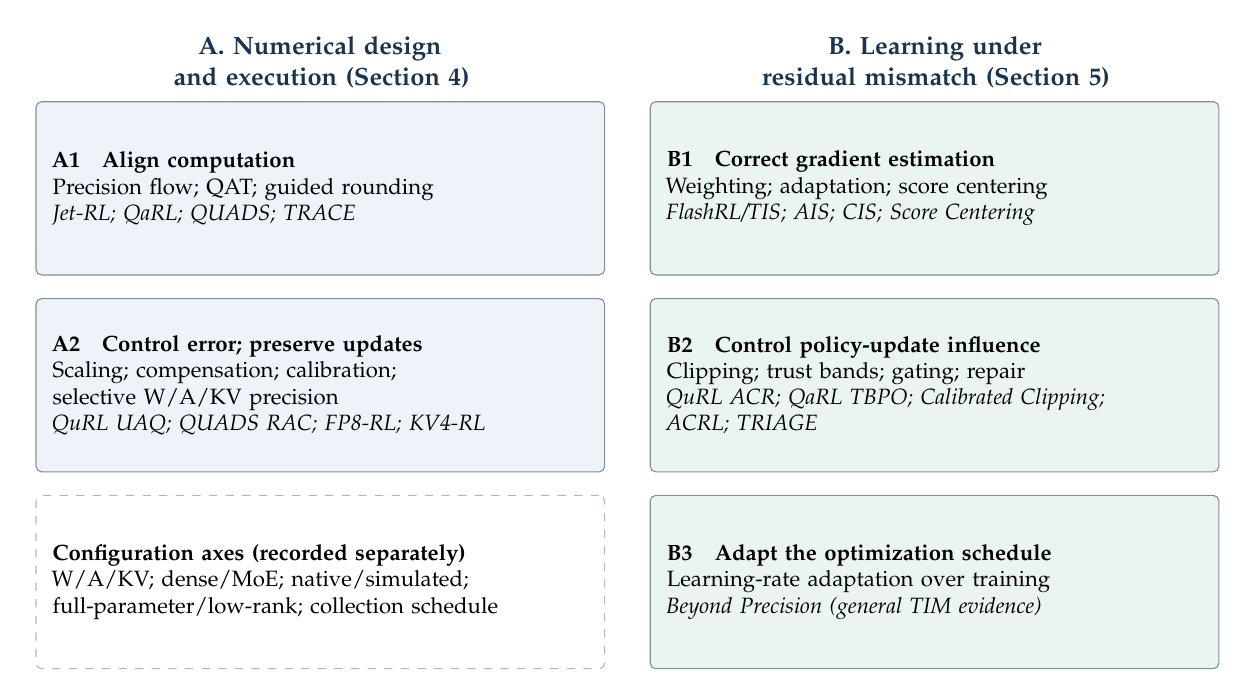
\begin{tikzpicture}[font=\footnotesize,>=Stealth,
 card/.style={draw=navy!55,rounded corners=2pt,align=left,text width=6.8cm,inner sep=6pt,minimum height=2.2cm},
 heading/.style={font=\small\bfseries,text=navy,align=center,text width=7.2cm}]
\node[heading] at (0,0) {A. Numerical design\\and execution (Section 4)};
\node[heading] at (7.8,0) {B. Learning under\\residual mismatch (Section 5)};
\node[card,fill=bluewash] at (0,-1.60) {\textbf{A1\quad Align computation}\\Precision flow; QAT; guided rounding\\\emph{Jet-RL; QaRL; QUADS; TRACE}};
\node[card,fill=bluewash] at (0,-4.10) {\textbf{A2\quad Control error; preserve updates}\\Scaling; compensation; calibration;\\selective W/A/KV precision\\\emph{QuRL UAQ; QUADS RAC; FP8-RL; KV4-RL}};
\node[card,fill=white,draw=navy!35,dashed] at (0,-6.60) {\textbf{Configuration axes (recorded separately)}\\W/A/KV; dense/MoE; native/simulated;\\full-parameter/low-rank; collection schedule};
\node[card,fill=tealwash] at (7.8,-1.60) {\textbf{B1\quad Correct gradient estimation}\\Weighting; adaptation; score centering\\\emph{FlashRL/TIS; AIS; CIS; Score Centering}};
\node[card,fill=tealwash] at (7.8,-4.10) {\textbf{B2\quad Control policy-update influence}\\Clipping; trust bands; gating; repair\\\emph{QuRL ACR; QaRL TBPO; Calibrated Clipping;\\ACRL; TRIAGE}};
\node[card,fill=tealwash] at (7.8,-6.60) {\textbf{B3\quad Adapt the optimization schedule}\\Learning-rate adaptation over training\\\emph{Beyond Precision (general TIM evidence)}};
\end{tikzpicture}
% END FIGURE taxonomy
\caption{Road map of the component taxonomy. Integrated studies can contribute components to both columns; configuration labels describe the experimental regime separately. The detailed taxonomy and evidence boundaries are developed in Sections~\ref{sec:form}, \ref{sec:numerical}, and~\ref{sec:learning}.}\label{fig:taxonomy-map}
\end{figure}

\subsection{Scope, Related Surveys, and Review Protocol}
Our focus is numerical and execution mismatch in LLM reinforcement learning, with emphasis on quantized rollout and closely related low-precision training configurations. We include asymmetric settings, such as a higher-precision learner with a lower-precision sampler, and settings in which both sides use low precision. Weight, activation, and key--value (KV) cache quantization are distinct numerical targets. Policy staleness is discussed where it interacts with execution mismatch, not treated as a synonym for it.

The review brings together twenty focal contributions: thirteen method or system studies, six studies that develop the formulation or analyze general mismatch, and one exploration-oriented boundary case. A supporting study can also provide direct low-precision evidence, as MiniRL does through its FP8-rollout experiments \citep{minirl}. Appendix~\ref{app:corpus} maps these contributions to their discussions, with conference and preprint versions treated as one work.

The literature snapshot is October 19, 2026. We follow a narrative review approach, developing a curated collection through targeted checks of primary papers; selection and version handling are described in Appendix~\ref{app:protocol}. General post-training quantization, pretraining-only methods, and speculative-draft acceleration fall outside the focal scope unless they directly clarify the learner--sampler interface.

Broader surveys cover low-precision LLM training, rollout strategies, and reinforcement learning for reasoning models \citep{lowprecisionsurvey,rolloutsurvey,reasoningsurvey}. Our emphasis is narrower: the relationship between actual sampling, numerical execution, and the update computed from sampled data. The exposition follows the component taxonomy developed below; numerical formats and experimental regimes are retained as separate comparison axes.

\subsection{Research Questions and Contributions}
Four questions guide the discussion: \textbf{RQ1}, how to separate execution mismatch from parameter changes and decoding differences; \textbf{RQ2}, how disagreement distorts estimation and optimization; \textbf{RQ3}, which objects numerical and learning interventions modify; and \textbf{RQ4}, which findings hold under the reported experimental conditions and system costs.

Our contribution is to connect policy semantics, intervention mechanisms, and published evidence. Sections~\ref{sec:form}--\ref{sec:mechanisms} establish a common notation and trace how execution differences enter learning (RQ1--RQ2). The component taxonomy then makes integrated methods comparable through the operations they change, organizing Sections~\ref{sec:numerical}--\ref{sec:learning} (RQ3). Section~\ref{sec:synthesis} relates the resulting learning outcomes to evaluation rules, information requirements, and cost (RQ4), leading to the research directions in Section~\ref{sec:open}.

\clearpage
\begingroup
\fontsize{9.5}{11}\selectfont
\setlength{\parskip}{0pt}
\setcounter{tocdepth}{2}
\makeatletter
\renewcommand*\l@section[2]{\addvspace{4pt}\@dottedtocline{1}{0em}{1.8em}{\bfseries #1}{\bfseries #2}}
\renewcommand*\l@subsection{\@dottedtocline{2}{1.8em}{2.5em}}
\tableofcontents
\makeatother
\endgroup
\clearpage

\section{Problem Formulation and Taxonomy}\label{sec:form}
\subsection{Learner, Behavior, Proximal, and Reference Policies}
Let $x$ be a prompt, $y_{1:T}$ a response, and $h_t=(x,y_{<t})$ its prefix. A policy is specified by both a parameter state and the computation used to evaluate it. Write $p_\theta(a\mid h)$ for the current learner policy and $p_k(a\mid h)$ for the same learner-side path at sampling snapshot $\theta_k$.

The behavior policy $q_k(a\mid h)$ is the distribution that actually sampled the token. It includes the rollout engine, numerical representation, and sampling transformation. Temperature and vocabulary truncation therefore belong to its definition: a raw-model log-probability returned by an engine need not equal the probability after decoding transformations.

The notation conditions on a documented collection protocol. With deterministic execution and version schedules, sampler cache state is determined by the generated history, even when some cache entries were computed under earlier parameter versions. The subscript $k$ abbreviates this specified rollout path; checkpoint identity alone is insufficient to reconstruct an unspecified stateful execution.

A proximal policy $p_{\mathrm{prox}}$ supplies the denominator of a policy-update constraint. A reference policy $p_{\mathrm{ref}}$ supplies a regularization target. These are different roles: a frozen pre-update learner may be proximal, while a much earlier policy is the KL reference. Neither is automatically the policy that generated every token. PPO and GRPO provide familiar contexts for these distinctions \citep{ppo,grpo}; mismatch-aware formulations require them to remain explicit \citep{flashrl,minirl}.

\begin{table}[!htbp]
\centering\small
\caption{Policies and quantities used throughout the survey. Execution paths are part of policy identity.}\label{tab:notation}
\begin{tabularx}{\linewidth}{@{}lY@{}}\toprule
Symbol & Meaning \\\midrule
$p_\theta$ & Current learner policy under its specified execution path.\\
$p_k$ & Learner-side policy evaluated at sampling snapshot $\theta_k$.\\
$q_k$ & Actual behavior policy that sampled the token.\\
$p_{\mathrm{prox}}$ & Policy used to define the proximal update ratio.\\
$p_{\mathrm{ref}}$ & Policy used for KL regularization; not the behavior denominator.\\
$\Delta_k$ & Same-snapshot log-probability difference, $\log p_k-\log q_k$.\\
$d_\theta$ & Current learner--behavior gap, $\log p_\theta-\log q_k$.\\
$A_t$ & Advantage or other policy-gradient learning signal.\\
$s_\theta(a,h)$ & Score vector, $\nabla_\theta\log p_\theta(a\mid h)$.\\\bottomrule
\end{tabularx}
\end{table}

\subsection{Execution Mismatch versus Policy Staleness}
At a fixed prefix and token with positive relevant probabilities,
\begin{equation}\label{eq:decomp}
\frac{p_\theta(a\mid h)}{q_k(a\mid h)}=
\underbrace{\frac{p_\theta(a\mid h)}{p_k(a\mid h)}}_{\text{parameter change}}
\underbrace{\frac{p_k(a\mid h)}{q_k(a\mid h)}}_{\text{same-snapshot execution/decoding difference}}.
\end{equation}
The factorization separates two comparisons at the same observed prefix. Its first factor measures parameter change since collection, including version lag in asynchronous execution; it requires no independence assumption. The snapshot policy $p_k$ is a conceptual same-parameter reference; an implementation need not retain it explicitly to use a different proximal policy. The second factor isolates numerical execution when decoding rules are controlled, and includes a decoding component when temperature or top-$p$ filtering differs. In partial rollouts, the sampling index may be token-dependent, $k=k(t)$. Moreover, carrying a cache across synchronization can preserve computations from earlier parameter states. In such an implementation, the current checkpoint index alone does not specify the behavior policy; cache provenance or the realized sampling probabilities are also needed. Cache retention is an implementation choice, so this qualification applies to implementations that carry those states across synchronization.

Two limiting cases make the distinction concrete. At the sampling snapshot, the learner-side parameter-change factor is one while execution mismatch can remain. With matched execution and decoding, the second factor can instead be one while policy lag remains. A numerical intervention and a staleness correction therefore solve different parts of the same ratio.

Probability ratios also require support conditions. A token observed from $q_k$ has a defined denominator, but that alone does not establish that $q_k$ covers every action with positive target probability. Truncation sampling can violate this condition. Similarly, a token-level change of measure is not automatically a correction for the prefix distribution. At fixed $h$,
\begin{equation}\label{eq:is}
\E_{a\sim q_k(\cdot\mid h)}\!\left[\frac{p_\theta(a\mid h)}{q_k(a\mid h)}f(a,h)\right]
=\E_{a\sim p_\theta(\cdot\mid h)}[f(a,h)]
\end{equation}
holds under support and integrability assumptions. It says nothing by itself about whether the outer distribution over $h$ is the desired one. It also does not undo changes to group-relative advantages induced by collecting different responses.

For comparison, the full-response likelihood ratio is
\begin{equation}\label{eq:trajectory}
W_\theta(y\mid x)=\frac{P_\theta(y\mid x)}{Q(y\mid x)}
=\prod_{t=1}^{T}\frac{p_\theta(y_t\mid h_t)}{q_{k(t)}(y_t\mid h_t)}.
\end{equation}
Here $P_\theta$ and $Q$ are the induced response laws, and the denominator factors must be their actual conditional probabilities under the documented protocol. Unobserved execution randomness requires marginalizing that state or extending the likelihood to the corresponding execution events. The two response laws use a common stopping convention; an end-of-sequence decision is included when applicable. For a fixed behavior law and a parameter-independent reward $R$, the usual likelihood-ratio identity gives
\begin{equation}\label{eq:seqpg}
\nabla_\theta\E_{P_\theta}[R]
=\E_Q\!\left[W_\theta R\sum_{t=1}^{T}s_\theta(y_t,h_t)\right]
\end{equation}
under support, integrability, and differentiation assumptions. The product illustrates why exact response-level correction can have high variance; multiplying only the current token ratio into an arbitrary sampled advantage is a different estimator. Nor does Equation~\eqref{eq:seqpg} directly justify reusing group-normalized advantages computed under $Q$. Score Centering explicitly distinguishes sequence-level importance sampling from practical token-level corrections \citep{score}.


\subsection{A Component-Level Taxonomy of Interventions}
We group components by the object they directly modify. \textbf{A: numerical interventions} alter representation or execution. A1 matches computation between learner and sampler; A2 controls quantization error or preserves parameter updates. \textbf{B: learning interventions} alter how sampled data produce updates. B1 corrects gradient estimation; B2 controls the acceptance, magnitude, or direction of policy updates; B3 adapts the optimization schedule.

These are organizing categories, not disjoint mathematical sets. Their boundaries answer an operational question: if the component is removed while the rest of the system is held fixed, which computation or update rule changes? An estimator correction changes an update, and an execution alignment can improve quantization fidelity. The primary assignment follows the component's operative rule and design objective. In particular, a multiplicative weight is not sufficient to identify importance sampling. We distinguish a weight constructed to correct a distributional estimation problem from a weight constructed to control how an update changes disagreement. Schedule adaptation is an emerging direction whose direct low-bit evidence remains limited.

\begin{table}[!htbp]
\centering\small
\caption{Five intervention classes. These categories describe operative components, not exclusive paper types.}\label{tab:taxonomy}
\begin{tabularx}{\linewidth}{@{}P{11mm}P{35mm}YY@{}}\toprule
Class & Direct object & Representative components & Important residual question\\\midrule
A1 & Shared computation & Precision flow; aligned QAT; guided rounding & Which interfaces remain unmatched?\\
A2 & Quantization fidelity & UAQ; residual compensation; calibration; selective precision & Are useful parameter changes visible?\\
B1 & Gradient estimator & TIS; AIS; CIS; Score Centering & Which expectation is corrected, and with what bias?\\
B2 & Update influence & ACR; TBPO; calibrated clipping; direction-aware controls & Which updates are retained or suppressed?\\
B3 & Optimization schedule & Mismatch-informed LR adaptation & Is stability obtained at comparable learning progress?\\\bottomrule
\end{tabularx}
\end{table}

\begin{figure}[!htbp]
\centering
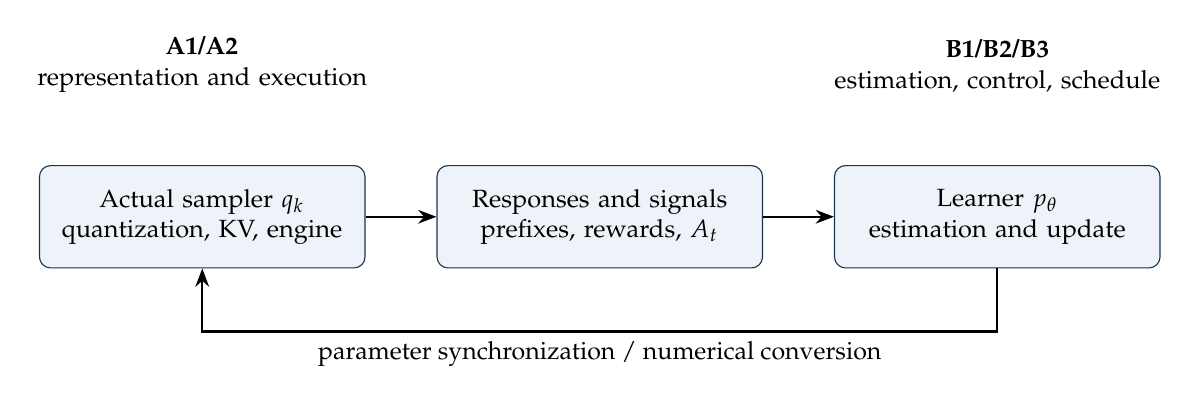
\begin{tikzpicture}[font=\small,box/.style={draw=navy,rounded corners,align=center,text width=39mm,minimum height=13mm,fill=bluewash},>=Stealth]
\node[box] (q) {Actual sampler $q_k$\\quantization, KV, engine};
\node[box,right=9mm of q] (data) {Responses and signals\\prefixes, rewards, $A_t$};
\node[box,right=9mm of data] (p) {Learner $p_\theta$\\estimation and update};
\draw[->,thick] (q)--(data);\draw[->,thick] (data)--(p);
\draw[->,thick] (p.south) -- ++(0,-8mm) -| node[pos=.25,below]{parameter synchronization / numerical conversion} (q.south);
\node[align=center,above=8mm of q,text width=42mm] {\textbf{A1/A2}\\representation and execution};
\node[align=center,above=8mm of p,text width=43mm] {\textbf{B1/B2/B3}\\estimation, control, schedule};
\end{tikzpicture}
\caption{The feedback loop reviewed in this survey. Numerical interventions may affect either execution endpoint; learning interventions act on the update. Arrows express data flow, not a claim that interventions must be applied in a particular order.}\label{fig:loop}
\end{figure}

\FloatBarrier
\subsection{Configurations and Evidence Labels}
The same intervention can operate under different numerical configurations. W/A/KV precision, dense versus mixture-of-experts (MoE) architecture, low-rank versus full-parameter updates, synchronous versus partial collection, and native kernels versus quantize--dequantize simulation are recorded separately. ``FP4 training'' does not specify which operations use FP4 or whether master weights, backward computation, and optimizer states remain at higher precision.

Contribution and evidence also deserve separate treatment. A formulation study can contain direct quantized-rollout experiments, while a quantized system can adopt an existing correction. Keeping those roles explicit preserves both relevant experiments and accurate attribution.

\section{Mechanisms: From Numerical Discrepancy to Learning Dynamics}\label{sec:mechanisms}
\subsection{Sources and Propagation of Execution Discrepancy}
A numerical policy is determined by more than its checkpoint. Scale selection, rounding, accumulation, kernel choice, batch shape, and the treatment of cached states can alter the output distribution. Sharing a nominal format therefore does not imply sharing a computation. FP16-based mismatch analysis provides a useful precision-selection comparison, while R3 exposes the importance of matching discrete routing decisions in MoE execution \citep{fp16,r3}. Neither should be treated as evidence that every routing discrepancy originates in quantization.

Two measurement settings must remain separate. \emph{Shared-prefix comparison} holds the token history fixed and compares conditional distributions. \emph{Free-running comparison} allows sampling differences to change the histories visited. The first is valuable for isolating a numerical interface; the second measures behavior after divergence has propagated through generation. A favorable shared-prefix statistic is not, on its own, a guarantee of similar trajectory-level learning signals.

Discretization introduces a further asymmetry. An update can be visible in the learner's parameter space but fail to change the sampler's quantized representation. Conversely, a small change near a rounding boundary can abruptly change a codeword. QuRL studies the former through update-aware quantization; TRACE targets inconsistency in rounding outcomes \citep{qurl,trace}. The relevant object is therefore not only error magnitude, but its relationship to the evolving parameters and the discretization boundaries.

\subsection{Distorted Estimation and Update Decisions}
At an observed prefix, numerical disagreement can change an update through its weight, its expected direction, or the clipping branch it activates. These mechanisms require different diagnostics. A probability difference and an importance ratio, for example, encode different information. Writing a learner probability as $p=q+\delta$ gives $p/q=1+\delta/q$: the same absolute perturbation has a larger relative effect when $q$ is small. This elementary observation motivates reporting tail behavior and confidence-conditioned statistics rather than only mean absolute probability error. CIS makes confidence dependence explicit in its correction design \citep{cis}.

Estimation can also acquire a systematic drift. For a normalized differentiable learner distribution, $\E_{a\sim p_\theta}[s_\theta(a,h)]=0$. Under behavior sampling, the corresponding expectation need not vanish. At fixed $h$,
\begin{equation}\label{eq:drift}
\E_q[A s_\theta]
=\operatorname{Cov}_q(A,s_\theta)+\E_q[A]\E_q[s_\theta].
\end{equation}
The expectations are conditional on the prefix and include the sampled action and any random continuation used to form $A$. Centering advantages across a prompt group need not center them at each prefix. Score Centering uses this distinction to motivate an additive correction \citep{score}: it removes a first-moment drift term while leaving the behavior distribution itself unchanged.

Mismatch additionally affects decisions made by a surrogate objective. In a clipped policy-gradient objective, changing a ratio can change which branch is active and therefore whether a token contributes gradient. Thus, a perturbation can matter through a threshold crossing even when its absolute magnitude appears modest. The full-pipeline FP8 study isolates a failure involving excessive clipping of negative-advantage tokens \citep{fullfp8}. This is a different intervention target from merely decreasing the variance of a sampled importance weight.

The sign dependence can be seen without assuming a particular quantizer. Let
$\ell(r,A)=\min\{rA,\clip(r,1-\epsilon,1+\epsilon)A\}$, with $0<\epsilon<1$ and fixed $A$. Away from the two boundaries,
\begin{equation}\label{eq:clipbranch}
\frac{\partial\ell}{\partial r}=
\begin{cases}
 A\,\mathbf{1}\{r<1+\epsilon\},& A>0,\\
 A\,\mathbf{1}\{r>1-\epsilon\},& A<0,\\
 0,&A=0.
\end{cases}
\end{equation}
Thus the active clipping side depends on the learning signal. For an illustrative objective that clips the combined learner--behavior ratio, a same-snapshot ratio of $0.7$ with $\epsilon=0.2$ already suppresses a negative-advantage token, even before a learner update. This is not the decoupled surrogate in Section~\ref{sec:b1}; the example explains why naming the clipped ratio is essential to interpreting a failure or a repair.



Figure~\ref{fig:clipping-sign} makes this sign dependence explicit for the standard surrogate. It also shows why clipping the combined learner--behavior ratio can suppress an update that a proximal ratio would still permit.

\begin{figure}[!htb]
\centering
% BEGIN FIGURE clipping
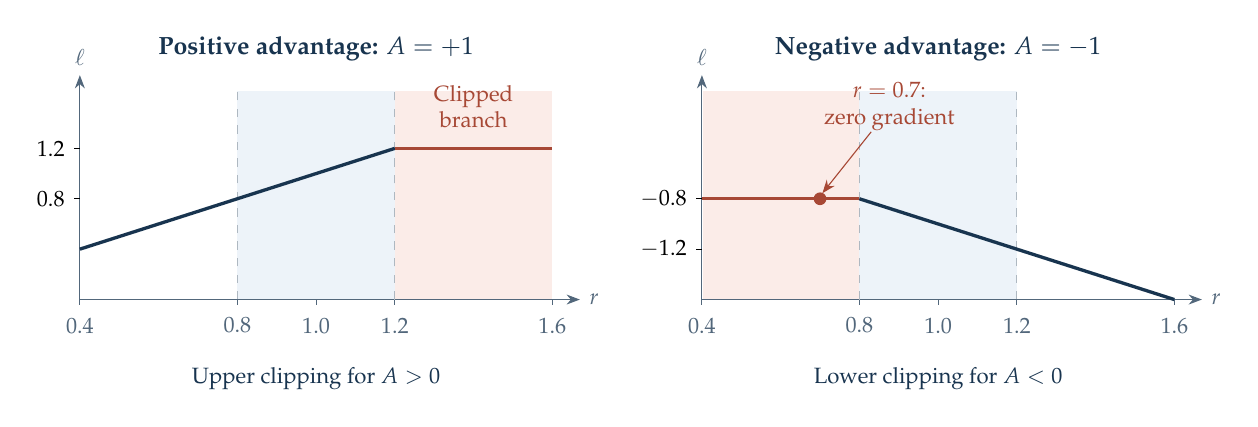
\begin{tikzpicture}[font=\footnotesize,>=Stealth]
\foreach \shift/\paneltitle in {0/{Positive advantage: $A=+1$},7.9/{Negative advantage: $A=-1$}}{
\begin{scope}[xshift=\shift cm]
\node[font=\small\bfseries,text=navy] at (3,3.18) {\paneltitle};
\fill[bluewash] (2,0) rectangle (4,2.65);
\draw[navy!35,dashed] (2,0)--(2,2.65);
\draw[navy!35,dashed] (4,0)--(4,2.65);
\draw[->,navy!75] (0,0)--(6.35,0) node[right] {$r$};
\draw[->,navy!75] (0,0)--(0,2.85) node[above] {$\ell$};
\foreach \x/\r in {0/0.4,2/0.8,3/1.0,4/1.2,6/1.6}{
\draw[navy!75] (\x,0)--(\x,-.07) node[below=1pt] {$\r$};}
\end{scope}}
\fill[redwash] (4,.01) rectangle (6,2.65);
\fill[redwash] (7.91,.01) rectangle (9.9,2.65);
\draw[navy!35,dashed] (4,0)--(4,2.65);
\draw[navy!35,dashed] (9.9,0)--(9.9,2.65);
\draw[very thick,navy] (0,.64)--(4,1.92);
\draw[very thick,redwarn] (4,1.92)--(6,1.92);
\draw[very thick,redwarn] (7.9,1.28)--(9.9,1.28);
\draw[very thick,navy] (9.9,1.28)--(13.9,0);
\draw (0,1.28)--(-.07,1.28) node[left] {$0.8$};
\draw (0,1.92)--(-.07,1.92) node[left] {$1.2$};
\draw (7.9,1.28)--(7.83,1.28) node[left] {$-0.8$};
\draw (7.9,.64)--(7.83,.64) node[left] {$-1.2$};
\fill[redwarn] (9.4,1.28) circle (2.3pt);
\draw[->,redwarn] (10.05,2.13)--(9.43,1.35);
\node[text=redwarn,align=center] at (10.28,2.45) {$r=0.7$:\\zero gradient};
\node[text=redwarn,align=center] at (5,2.45) {Clipped\\branch};
\node[align=center,text=navy] at (3,-1.0) {Upper clipping for $A>0$};
\node[align=center,text=navy] at (10.9,-1.0) {Lower clipping for $A<0$};
\end{tikzpicture}
% END FIGURE clipping
\caption{Analytical illustration of Equation~\eqref{eq:clipbranch} with $\epsilon=0.2$ and $A=\pm1$. Blue shading marks $[0.8,1.2]$; red shading marks the flat, clipped branch. A ratio of $0.7$ lies on the zero-gradient branch for negative advantage. The relevant interpretation depends on which policy ratio the objective clips.}\label{fig:clipping-sign}
\end{figure}

\subsection{Feedback across Optimization Steps}
The learning loop turns a local discrepancy into a dynamic process. A sampled response changes the learner; the learner is synchronized back to the sampler; the next rollout is then generated from an updated numerical realization. Stability depends on this feedback, not solely on whether one frozen batch has a small error.

Direction matters because two updates with the same gap magnitude can move learner and behavior probabilities differently. In a simplified local picture, reducing a learner probability that is already below the behavior probability can enlarge their log gap. ACRL and TRIAGE use update-direction information in their controls \citep{acrl,triage}. For a shared-parameter network, however, one token's update changes other probabilities too. The sign argument supplies local intuition; interactions through shared parameters determine the scope of any stability result.

Optimization scale adds another feedback channel. Beyond Precision studies the relationship between mismatch and optimization dynamics and proposes response-length-triggered learning-rate decay \citep{beyond}. This connects numerical observations to the scale of optimization, while leaving transfer of the schedule to aggressive FP4 execution open.

\subsection{Diagnosing the Effects of Mismatch}
Diagnosis begins with the comparison used to isolate an effect. Replacing an inference engine can simultaneously change arithmetic, batching, memory use, and generated trajectories. A resulting quality difference cannot automatically be assigned to the precision format. VeXact constructs a zero-mismatch reference to help separate execution mismatch from other training effects \citep{vexact}. It supplies a diagnostic counterfactual against which the effects of accelerated execution can be interpreted.

The evidence chain has three links: an execution change alters conditional probabilities; those probabilities alter the estimator or update decision; repeated updates alter the learned policy. Shared-prefix replay can isolate the first link, update diagnostics probe the second, and training trajectories establish the third under a stated horizon. An ablation that identifies one link is valuable, but leaves the others to be established. Section~\ref{sec:synthesis} follows these links when drawing together the published findings.

\discussion{Box 1. Does smaller mismatch always mean better learning?}{QeRL combines low-precision execution, low-rank adaptation, and adaptive quantization noise, making exploration an explicit part of its setting \citep{qerl}. It is a boundary case for this survey, not a method for eliminating mismatch. Its results motivate separating numerical agreement from task utility, but do not imply that arbitrary cross-engine error is beneficial. A useful comparison must ask what changed in the sampling distribution, what adaptation capacity the learner had, and whether the gain persists under matched evaluation.}

\takeaway{Mismatch is not one scalar defect. Conditional probability error, trajectory selection, estimator drift, threshold decisions, and cross-step feedback are distinct objects. A method should be assessed against the object it actually changes.}

\section{Numerical Design and Execution Alignment}\label{sec:numerical}
Numerical design offers two complementary ways to change the policy that generates training data. Alignment brings learner and sampler computations closer at a shared interface; fidelity control preserves the information that a low-precision representation would otherwise lose. The distinction matters because two approximate paths can agree without either becoming more accurate relative to a higher-precision model.

\subsection{Aligning Learner and Rollout Computation}\label{sec:a1}
Jet-RL moves the discussion from matching bit widths to matching precision flow \citep{jet}. Its unified FP8 design coordinates the numerical paths and quantization granularity used by learner and sampler. Agreement is pursued through corresponding operators, rather than inferred from an FP8 label alone. This path-level view provides a starting point for later approaches that couple the endpoints more selectively.

QaRL implements such coupling through rollout-aligned quantization-aware training (QAT): the learner's forward pass reflects the representation used during generation \citep{qarl}. QUADS takes a deliberately asymmetric approach, fake-quantizing learner weights while retaining higher-precision learner activations \citep{quads}. Both designs bring part of the learner computation closer to the sampler, but QUADS leaves activation error to a separate rollout-side component. Their comparison reveals that alignment can be selective; uniform precision across the whole model is neither its definition nor a prerequisite. QAT emulation and native low-precision kernels nevertheless remain distinct numerical paths.

TRACE goes further by sharing realized quantization information \citep{trace}. It records compact rollout-side information to guide learner-side FP4 rounding, addressing cases in which a common quantizer specification still produces different decisions near a rounding boundary. Its local rounding argument explains this interface-level benefit without establishing monotonic reduction of full-network policy divergence.

These approaches couple the endpoints through increasingly specific information: a precision-flow design, an emulated representation, or realized numerical decisions. They represent different choices about what to share, rather than successive points on a universal performance ranking. Routing replay follows a related principle for discrete MoE execution choices \citep{r3}. As coupling becomes more specific, correspondence between token positions, modules, and parameter versions becomes part of the method's validity. The remaining computation still determines how closely the complete policies agree.

\subsection{Controlling Quantization Error and Preserving Parameter Updates}\label{sec:a2}
Alignment alone does not ensure that the sampler can express the changes made by training. For an illustrative deterministic quantizer $Q$, an update can satisfy
\begin{equation}\label{eq:quantupdate}
Q(w+\delta w)=Q(w),
\end{equation}
even when $\delta w\ne0$. Visibility depends on the distance to a quantization boundary and on scale behavior, as well as update magnitude. QuRL's Update-Aware Quantization uses invariant scaling to alter the relationship between quantization resolution and parameter updates \citep{qurl}. Its numerical contribution is therefore distinct from ACR, which modifies the clipping rule in Section~\ref{sec:b2}.

QUADS addresses another residual: activation error in the rollout path. Its Residual Activation Compensation complements learner-side weight QAT, allowing alignment and error reduction to operate on different parts of the system \citep{quads}. The component ablations are particularly useful here because they distinguish what weight alignment recovers from what activation compensation adds.

Maintaining fidelity also requires following a changing policy. FP8-RL integrates blockwise W8A8 rollout, scale recalibration for FP8 attention and KV execution, and dynamic weight synchronization \citep{fp8rl}. The contribution lies in keeping these numerical components operational throughout RL, together with adopted TIS/MIS correction. Its v2 experiments also explore end-to-end FP8, making learner precision an experiment-level attribute rather than a fixed description of the entire paper.

KV4-RL allocates fidelity across positions instead of raising precision uniformly \citep{kv4}. INT4 KV storage is supplemented by bounded INT8 protection for attention-sink and recent positions. Its retained TIS recipe makes the distinction between sampler fidelity and conditional correction especially clear: protecting the cache changes the data-generating computation even when the correction is held fixed. The experiments use colocated, quota-based partial collection, with generation and optimization alternating; responses may span collection boundaries.

Across these studies, the useful precision budget is the one that preserves information relevant to learning. Parameter rescaling protects update visibility, residual compensation addresses activation error, recalibration follows distributional change, and positional protection targets sensitive cache states. W/A/KV identifies where these mechanisms operate; it does not replace the distinction between them.

\subsection{Residual Mismatch and Limits of Alignment}
The scope of alignment follows its interface. Matching weights can leave activation differences; matching a quantizer can leave different surrounding kernels; protecting selected states can leave the rest of the network unchanged. Agreement and fidelity are therefore separate achievements, each tied to a parameter snapshot and input history.

This partial coverage explains why numerical methods often coexist with learning correction. A more faithful sampler can still lag behind the learner, while a closely matched conditional distribution cannot undo the histories excluded by earlier sampling decisions. The residual determines what a learning-side intervention has left to address.

\takeaway{Numerical methods differ in what they share and what they preserve. Their effect on learning depends on the protected interface, the remaining discrepancy, and the cost of maintaining that relationship.}

\section{Learning under Residual Mismatch}\label{sec:learning}
Learning interventions accept that the rollout data and learner computation may differ. Their goals range from adjusting an estimator to controlling harmful updates or changing the optimization schedule. They should not all be evaluated as approximations to the same unbiased gradient: some deliberately modify the update to trade bias, variance, or stability against one another.

\subsection{Correcting Gradient Estimation}\label{sec:b1}
\paragraph{Multiplicative correction and truncation.}
Importance sampling supplies a conditional change of measure under the assumptions of Equation~\eqref{eq:is}. Practical surrogate objectives usually distinguish the mismatch correction from the proximal update ratio. With frozen $p_{\mathrm{prox}}$ and recorded behavior $q$, define
\begin{equation}\label{eq:tworatios}
c_t=\frac{p_{\mathrm{prox}}(a_t\mid h_t)}{q(a_t\mid h_t)},\qquad
r_t(\theta)=\frac{p_\theta(a_t\mid h_t)}{p_{\mathrm{prox}}(a_t\mid h_t)}.
\end{equation}
A representative decoupled surrogate is
\begin{equation}\label{eq:surrogate}
\widehat L(\theta)=\frac1N\sum_t \sg(\bar c_t)
\min\!\left[r_t(\theta)A_t,\clip(r_t(\theta),1-\epsilon,1+\epsilon)A_t\right],
\end{equation}
where $\bar c_t$ is a possibly truncated correction, the sampled advantages are held fixed, and $\sg$ denotes no differentiation through the correction weight. This is a schematic comparison device, not a claim that every reviewed method implements Equation~\eqref{eq:surrogate} identically. It separates two operations: bounding the correction $c_t$ and clipping the proximal ratio $r_t$. An upper-truncated correction, for example, takes $\bar c_t=\min(c_t,C)$, whereas masking can discard selected ratios. Here $N$ counts valid sampled tokens; response-level averaging or length normalization changes their relative weights and must be retained when comparing implementations.

FlashRL's TIS provides a basic bounded correction using actual rollout probabilities \citep{flashrl}. MiniRL exemplifies the mismatch-aware distinction between behavior and proximal policies underlying this notation \citep{minirl}. FP8-RL adopts token-level TIS/MIS variants, while KV4-RL retains TIS alongside cache protection \citep{fp8rl,kv4}. These uses contribute system evidence without creating additional estimator families. Truncation limits extreme influence but changes the expectation. A stable truncated objective should therefore not be described as exact importance sampling merely because its denominator comes from the sampler.

\paragraph{Adapting the amount and location of correction.}
AIS uses observable mismatch diagnostics to interpolate between uncorrected and fully importance-weighted gradients \citep{ais}. Its adaptive quantity is the estimator mixture, not a precision schedule. CIS instead derives a confidence-dependent importance-weight cap from a discrepancy representation \citep{cis}. These approaches differ in what they adapt: overall correction strength versus the location of truncation across token confidence. CIS is used here as general TIM evidence; its BF16 cross-engine experiments are not direct FP4 validation.

\paragraph{Additive score correction.}
Score Centering replaces the score at a prefix with
\begin{equation}\label{eq:center}
\widetilde s_\theta(a,h)=s_\theta(a,h)-\E_{b\sim q(\cdot\mid h)}[s_\theta(b,h)].
\end{equation}
With the exact expectation, its mean under $q$ vanishes and the drift term in Equation~\eqref{eq:drift} is removed \citep{score}. The remaining covariance is still measured under $q$, so this is not full recovery of an on-policy gradient. The reported implementation uses sampler top-$k$ log-probabilities and models the omitted tail using the learner distribution; its default is $k=128$ \citep{score}. The resulting approximation is more specific than simply discarding the tail. Its coefficients are detached when forming the correction, and its fidelity depends on the reconstructed behavior distribution.

The distinction between multiplicative and additive correction also determines the information returned by the sampler. Ratio-based methods need probabilities of sampled actions; exact score centering needs a behavior-weighted score expectation. Truncation and reconstruction make different approximations to these quantities. Their derivative interpretation additionally depends on the learner computation, including any surrogate gradient through a quantizer.

\subsection{Controlling the Influence of Policy Updates}\label{sec:b2}
\paragraph{Restoring or reshaping update constraints.}
QuRL's Adaptive Clipping Range adjusts the update boundary in response to the relationship between proximal and behavior probabilities \citep{qurl}. QaRL's TBPO combines negative-sample treatment with sequence-level trust-band control \citep{qarl}. The full-pipeline FP8 method first matches the lower clipping quantile on negative-advantage tokens to a BF16 reference, then adjusts the upper boundary to rebalance positive and negative contributions \citep{fullfp8}. Periodic reference passes amortize the calibration cost. All three act on the update constraint, but use different signals and aggregation levels. ``Calibration'' in the last method refers to objective boundaries, not quantizer scales.

The shared issue is which learning signal reaches the parameter update. A token-level boundary can restore a contribution lost to clipping, whereas a sequence-level trust band controls a whole response. Widening either region admits more updates, but their value depends on advantage sign and influence. The clipping count becomes informative when connected to those retained contributions.

\paragraph{Controlling disagreement through update direction.}
ACRL uses advantage-guided probability adjustment, with response-level discrepancy relative to a reference controlling token reweighting \citep{acrl}. Its objective is regulation, not unconditional minimization of discrepancy. TRIAGE instead combines segment-local risk information, direction-selective gating, rebalancing, and bounded repair in native NVFP4 execution \citep{triage}. Their common placement in B2 reflects the role of the update rule, not equivalence of their risk models or experimental settings.

The granularity of control matters. A response-level statistic aggregates evidence across many tokens; a segment statistic can expose local concentration; a token rule is directly selective but may be sensitive to noise. Aggregation trades localization against statistical reliability. Finer granularity improves localization only when the resulting diagnostic remains reliable enough to guide the update.

\subsection{Adapting the Optimization Schedule}\label{sec:b3}
A third intervention changes the scale of learning over time. Beyond Precision motivates learning-rate scheduling through the evolution of optimization and mismatch \citep{beyond}. This is complementary to changing a numerical path or a token weight: it modifies the trajectory of parameter updates themselves.

Schedule adaptation remains less developed for direct low-bit settings than the estimator and update controls above. Its promise depends on preserving progress as well as stability: smaller steps can avoid divergence while delaying useful learning. Comparable quality within a comparable budget is therefore the relevant test of transfer to aggressive quantization.

\subsection{Compatibility, Bias, and Failure Modes}
Several designs already combine numerical and learning components. QaRL, QuRL, and QUADS provide evidence for the combinations studied within each system; Score Centering describes composition with importance weighting by centering the weighted score \citep{qarl,qurl,quads,score}. These results motivate composition while leaving its behavior under other combinations open.

Compatibility depends on more than category membership. Components must refer to the same behavior policy and parameter snapshots, act coherently on the target estimator, and obtain their required information at acceptable cost. A centering term for one estimator need not center a differently weighted score; successive masks can remove the same examples; a reference pass can change the cost of an otherwise inexpensive rule. Section~\ref{sec:synthesis} relates these dependencies to the published system evidence.

The residual error helps explain where composition has value. Conditional correction leaves the collected histories unchanged, numerical alignment leaves policy lag, and clipping controls influence without reproducing the sampler's arithmetic. Combining components is useful when their remaining errors complement one another and the joint rule preserves enough signal to learn.

\takeaway{Estimator correction changes an expectation; update control changes which contributions are allowed to act; scheduling changes their evolution over training. Their composition depends on shared probability semantics and the learning signal that survives.}

\section{Synthesis of Findings and Practical Trade-offs}\label{sec:synthesis}
The literature offers its clearest comparisons through controlled changes within a system. Read together, these studies reveal how numerical fidelity, estimator behavior, and update selection interact. The synthesis below follows those connections, relating learning outcomes to the information and execution cost required to obtain them.

\subsection{Coverage of Existing Studies}
The corpus spans several configurations that should remain distinct. Asymmetric learner--sampler precision emphasizes a gap between numerical representations. Low precision on both sides emphasizes the consistency of their execution paths and the behavior of the resulting update. KV-focused work changes a state-storage interface, while weight or activation quantization changes other parts of computation. Low-rank adaptation and full-parameter RL additionally differ in which degrees of freedom can respond to quantization.

The autoregressive equations in Sections~\ref{sec:form}--\ref{sec:learning} describe token-generation paths. AIS also evaluates diffusion-based LLaDA alongside autoregressive Qwen models \citep{ais}. Its denoising experiments extend the empirical scope of the source, but require a generation-process-specific likelihood interpretation; they are not additional validation of the autoregressive factorization as written here. We use its autoregressive evidence for direct comparison in that formulation.

Architecture and collection protocol further condition conclusions. MoE execution introduces discrete route choices; cache-heavy long responses expose different runtime bottlenecks from shorter generations; partial collection permits a response to contain tokens sampled under different parameter versions. A method evaluated in one of these regimes may motivate a hypothesis in another, but that transfer is not itself an experimental result.

Appendix~\ref{app:corpus} maps the focal studies to their detailed discussions. The companion catalog records numerical configurations and source versions, while the evidence file links observations from all thirteen core method/system studies to the relevant source sections. Table~\ref{tab:observations} draws out six comparisons that most directly illuminate the findings below.

\subsection{Findings on Stability and Learning Quality}
Three findings connect studies that otherwise differ in format, architecture, and correction rule.

\paragraph{Correction must be evaluated over the learning trajectory.}
QuRL shows why an initially stable correction can be an incomplete account of a run: disagreement grows over a longer horizon, while ACR and UAQ address different changes in clipping and update visibility \citep{qurl}. AIS adapts the correction mixture, ACRL regulates discrepancy through update influence, and Score Centering targets an estimator drift term \citep{ais,acrl,score}. The common lesson is temporal: the distribution, correction, and learner evolve together. Early agreement or bounded weights describe only part of that evolution; the resulting update and quality trajectory establish whether the intervention remains useful.

\paragraph{Numerical coupling is useful at a specified interface.}
Jet-RL couples precision flow, while QaRL, QUADS, and TRACE couple representations or realized rounding decisions \citep{jet,qarl,quads,trace}. QUADS gives a particularly informative component comparison: asymmetric weight QAT recovers much of the learning loss, and rollout-side residual compensation improves the remaining gap. Its asymmetric-versus-symmetric QAT comparison further separates nominal symmetry from effective alignment. FP8-RL adds the system perspective, showing how calibration and synchronization support a changing low-precision policy \citep{fp8rl}. Together, these studies locate the benefit in a specified interface. Transfer depends on whether another stack preserves that interface and the surrounding computation.

\paragraph{Which updates survive can matter as much as average disagreement.}
The full-pipeline FP8 study connects excessive lower-side clipping of negative-advantage tokens to pathological training dynamics, whereas TRIAGE uses local and direction-dependent information to select interventions \citep{fullfp8,triage}. Both connect stability to the signed learning signal that remains after control, revealing structure hidden by an aggregate clipping fraction or mean log-probability gap. TRIAGE also limits token-wise directional predictiveness in its MoE routing-conditioned analysis, underscoring the difference between a population pattern and a reliable predictor for each token.

\begin{table}[!htb]
\centering\small\setlength{\tabcolsep}{4pt}
\caption{Selected published observations and their interpretive limits. These within-paper comparisons illustrate the synthesis; the twenty-work coverage map appears in Appendix~\ref{app:corpus}. No row defines a performance ranking across papers.}\label{tab:observations}
\begin{tabularx}{\linewidth}{@{}P{32mm}YY@{}}\toprule
Study / setting & Published comparison or observation & What the evidence supports \\\midrule
QuRL \citep{qurl}\newline INT8/FP8 rollout & Longer-run behavior differs from early TIS behavior; ACR and invariant-scaling ablations address distinct failure modes. & Correction magnitude, clipping semantics, and update visibility are separate concerns; a short stable window is insufficient.\\[3pt]
QUADS \citep{quads}\newline NVFP4 MoE rollout & Weight-only learner QAT recovers much of the loss; adding rollout activation compensation further improves held-out scores. & The two components have complementary evidence within this design; neither universal necessity nor cross-engine transfer follows.\\[3pt]
Score Centering \citep{score}\newline BF16 learner; quantization or lag & Shared-objective experiments compare additive centering and importance correction; their composition helps in the reported staleness tests. & Estimator drift and importance-weight control are distinguishable. The implemented behavior expectation is approximated.\\[3pt]
Full Pipeline FP8 \citep{fullfp8}\newline FP8 learner and rollout & Calibrated Clipping improves the reported learning outcomes across scaling choices. Main GRPO results use best-checkpoint selection over 500 steps. & Restoring signed update contributions can matter; the selected endpoint is not a fixed-budget final-checkpoint comparison.\\[3pt]
TRIAGE \citep{triage}\newline Native NVFP4 & Local tail patterns motivate direction-selective gating and repair. Token-wise predictiveness has a narrower scope than the population characterization. & Local and signed diagnostics can be informative, with limits under MoE coupling; token-independent contraction is not established.\\[3pt]
KV4-RL \citep{kv4}\newline INT4 KV; partial collection & Unprotected INT4 KV misses later learning gains under the retained TIS recipe; bounded INT8 protection recovers near-BF16 endpoint quality. & Conditional correction and cache fidelity address different effects. Timing and quality claims apply to the studied collection workload.\\
\bottomrule
\end{tabularx}
\end{table}

These findings connect fidelity and correction through the learning signal they preserve. Better execution can change which tokens require correction; a better update rule can make residual execution error tolerable. The strongest evidence links a component ablation to both the proposed mechanism and a learning outcome. This connection is what turns numerical agreement into a claim about effective training.

\subsection{Efficiency Gains and Implementation Costs}
The same complementarity has a system cost. For serialized phases, iteration time can be decomposed as
\begin{equation}\label{eq:time}
T_{\mathrm{iter}}=T_{\mathrm{rollout}}+T_{\mathrm{learner}}+T_{\mathrm{sync}}+
T_{\mathrm{quant/calib}}+T_{\mathrm{other}},
\end{equation}
where synchronization and quantization/calibration costs are separated from generation and learning. Accelerating one phase exposes the others. With overlapping execution, the relevant quantity is the critical path, so the phase times in Equation~\eqref{eq:time} cannot simply be added.

Each intervention changes a different part of this cost. FP8-RL illustrates the work needed for scale estimation and numerical conversion \citep{fp8rl}. Reference calibration adds learner computation; guided rounding adds storage, transport, and state matching; selective precision adds work in the protected region. Table~\ref{tab:interfaces} relates these dependencies to the information each method needs.

Token throughput also depends on the realized workload. A policy that produces shorter responses can appear faster without improving execution per token; one that produces longer responses can incur more work despite a faster kernel. Memory savings can increase concurrency, which changes the workload seen by attention and compute kernels. Serving research such as PagedAttention provides background for why cache management and scheduling affect observed throughput \citep{pagedattention}, but serving speed alone does not establish RL learning efficiency.

\begin{table}[!htbp]
\centering\small
\caption{Information and implementation requirements that distinguish the reviewed approaches. Entries describe method interfaces rather than measured overhead rankings.}\label{tab:interfaces}
\begin{tabularx}{\linewidth}{@{}P{32mm}YY@{}}\toprule
Approach & Information or execution dependency & Question for the system comparison\\\midrule
TIS / AIS / CIS & Behavior probabilities and learner/proximal probabilities & Are the stored probabilities those of the actual sampling distribution?\\
Score Centering & A behavior-weighted score expectation, exact or approximated & What distributional information is returned, and what approximation is used?\\
Aligned QAT & A learner path corresponding to rollout quantization & Which kernels and numerical interfaces remain different?\\
Guided rounding & Realized rollout-side quantization information & How are states stored, transferred, and matched to training?\\
Calibrated Clipping \citep{fullfp8} & Higher-precision reference ratios at calibration points & Is the reference-pass cost included in training time?\\
Selective KV precision & Low-bit cache execution with protected positions & Is protection cost bounded, and under which context workload?\\\bottomrule
\end{tabularx}
\end{table}

KV4-RL provides a concrete example of distinct timing scopes: over 400 iterations on Qwen3-8B-Base, it reports $1.80\times$ cumulative rollout speedup and $1.27\times$ cumulative full-iteration speedup over BF16 rollout \citep{kv4}. The two quantities describe the same study, yet already differ substantially. Its common-BF16 evaluation separates learned-policy comparison from evaluation precision. These figures illustrate timing scope rather than a comparison with another paper's hardware or workload.

Time or compute to a specified quality level connects these system measurements to the learning objective. Endpoint scores, iteration time, and rollout throughput each supply part of that picture. Recovering time-to-quality additionally requires the training trajectory, especially when an intervention changes response length, learning speed, or checkpoint selection.

\begin{table}[!htbp]
\centering\small
\caption{Conditions governing the interpretation of published learning and efficiency results.}\label{tab:evidence}
\begin{tabularx}{\linewidth}{@{}P{33mm}YY@{}}\toprule
Reported outcome & Conditions of comparison & Scope of interpretation\\\midrule
Smaller mismatch & Same parameters, prefixes, decoding rules, metric definition & Measures conditional agreement; stability requires learning evidence.\\
Stable training & Horizon, seeds, stopping criteria, quality trajectory & Establishes behavior over the observed horizon and budget.\\
Comparable accuracy & Evaluation precision, tasks, budget, checkpoint selection & Depends on the evaluation policy and checkpoint rule.\\
Faster rollout & Tokens, lengths, concurrency, hardware, baseline & Measures generation; full training includes other phases.\\
Lower memory & W/A/KV scope, allocated vs resident memory, batch policy & Throughput also depends on scheduling and concurrency.\\
Method combination & Joint ablation, estimator definitions, additional cost & Supports the joint rule under the tested conditions.\\\bottomrule
\end{tabularx}
\end{table}

\subsection{Limitations of Current Evidence}
The principal limitation is transfer across experimental settings. Training horizons, model families, tasks, and hardware differ, making controlled ablations within a study more informative than absolute results across unrelated systems. Mathematical reasoning is a recurring evaluation setting; long interactive trajectories and broader task distributions remain less directly covered. Numerical transfer is equally conditional: format, scaling, higher-precision exceptions, and kernels jointly define the execution path.

The survey inherits these limits and those of its curated narrative scope. The source-linked catalog makes the basis of each observation visible, but provides neither exhaustive retrieval nor independent replication. Where a source leaves an implementation or evaluation condition unreported, that uncertainty remains part of the comparison.

\takeaway{Published evidence most clearly supports relationships between mechanisms and outcomes under stated conditions. Linking numerical agreement, stable updates, policy quality, and runtime is the central task of synthesis.}

\section{Open Problems}\label{sec:open}
The preceding findings point toward a more predictive account of low-precision RL: one that explains when a discrepancy becomes harmful, which intervention is sufficient, and how its benefit survives a change of system or task.

\subsection{Predicting Harmful Mismatch}
Mean disagreement is an incomplete predictor because learning depends on where error occurs and which update it changes. Confidence-conditioned tails, signed clipping distortions, conditional drift, and directional concentration offer more specific candidates. The unresolved step is to connect these quantities to future learning damage before a task score reveals it.

A predictor of collapse within a horizon need not predict reduced improvement per update or failure to reach a quality threshold. Establishing its target makes the result interpretable. Transfer is the stronger test: a diagnostic that remains predictive after changing the correction or model is more likely to identify a mechanism than a feature of one training recipe. Intervention sensitivity is equally informative. When a control lowers the metric without improving learning, the relationship may be correlational or the control may suppress useful signal along with the risk.

\subsection{Composing Numerical and Learning Interventions}
Numerical fidelity changes the operating regime of a correction. Conversely, a correction that suppresses updates can change the apparent value of finer quantization. Their joint design therefore depends on marginal benefit: how much additional learning a component preserves after another component has already acted.

This interaction is especially delicate when multiple masks, truncations, or trust bands affect the same examples. An apparently stable combination can owe its behavior to weak learning. A useful account of composition would connect the joint estimator to the signed signal that survives, then relate that signal to quality gained per unit of computation. The information exchanged between endpoints belongs in the same comparison, since a statistically attractive correction may require expensive reference or distributional computations.

\subsection{Precision, Staleness, and Long-Horizon Interaction}
Partial and asynchronous collection can make the sampling version token-dependent. A probability gap may then combine parameter change with execution mismatch, as Equation~\eqref{eq:decomp} makes explicit. Separating their effects requires information about snapshots, replay, or retained cache states that a production system may not store. The smallest behavior record sufficient for reliable correction remains a joint statistical and system question.

Long responses amplify this difficulty. An early numerical perturbation changes the prefixes visited later, even if conditional correction at each observed prefix is accurate. This suggests allocating precision according to position, layer, context, and training phase, with learning benefit as the objective. Local tensor error alone cannot identify where the extra fidelity is worth its cost.

Multi-turn interaction extends the same question beyond token prefixes. Tool observations and environment transitions add state that shapes later behavior and may need to enter the record alongside cache provenance and sampling probabilities. The taxonomy still locates numerical and learning interventions, but evidence from single-response generation leaves their effectiveness in these settings open.

\subsection{Generalization and Comparable Evidence}
Transfer becomes easier to assess when results identify the learner and sampler paths, actual behavior probabilities, update ratios, collection schedule, evaluation precision, and timing scope. These details explain why two nominally identical precision settings can behave differently. They also distinguish an adopted algorithm from a system's integration contribution and native arithmetic from quantization emulation.

A shared vocabulary would allow results to accumulate across diverse evaluations. Learning trajectories and explicit checkpoint rules connect stability to quality; phase timing connects kernel gains to training cost; joint ablations connect component mechanisms to effective combinations. A universal benchmark is unnecessary for this narrative synthesis, but comparable evidence is essential to turning promising individual designs into transferable principles.

\section{Conclusion}\label{sec:conclusion}
Quantized rollout changes the computation that generates reinforcement-learning data, allowing numerical approximation to return through policy updates and future trajectories. Its consequences become clearer when execution mismatch is separated from policy staleness, and conditional correction from changes in the histories that are sampled.

The reviewed methods respond at complementary interfaces. Numerical alignment shares computation; fidelity control preserves sensitive information and parameter changes; estimator correction and update control determine how residual mismatch enters learning. Schedule adaptation adds a broader optimization perspective, with direct low-bit evidence still emerging. Across these approaches, the most useful comparisons connect a named mechanism to the learning signal it preserves and the cost of preserving it.

This perspective shifts attention from reducing a single discrepancy statistic to understanding effective learning under approximate execution. Predictive diagnostics, coherent method composition, and explicit behavior semantics can help the field move from successful individual configurations toward principles that transfer across models, numerical paths, and interaction settings.

\clearpage
\appendix
\section{Focal Corpus and Section Mapping}\label{app:corpus}
The following table contains twenty unique focal contributions. A primary location identifies where a work is developed in detail; additional locations identify a distinct component or a contextual use. Supporting roles do not imply absence of direct low-precision experiments. Conference and preprint versions are not counted twice. Foundational and neighboring references are excluded from the count of twenty.
\begingroup\footnotesize\setlength{\tabcolsep}{4pt}
\begin{longtable}{@{}P{29mm}P{22mm}P{23mm}P{71mm}@{}}
\caption{Focal works, component classes, and primary discussion locations. Secondary locations are shown in parentheses. All twenty enter the literature coverage synthesis.}\label{tab:corpus}\\
\toprule Work & Class / role & Location & Scope note \\\midrule\endfirsthead
\toprule Work & Class / role & Location & Scope note \\\midrule\endhead
\midrule\multicolumn{4}{r}{Continued on next page}\\\endfoot
\bottomrule\endlastfoot
FlashRL / TIS \citep{flashrl} & B1 & 5.1 (1.1; 2.1) & Quantized rollout; recorded behavior probabilities. \\
QeRL \citep{qerl} & Boundary & Box 1 & NVFP4 with LoRA and adaptive noise; exploration setting. \\
Jet-RL \citep{jet} & A1; A2 & 4.1 (6.2) & Unified FP8 flow; granularity is an associated numerical design choice. \\
FP8-RL \citep{fp8rl} & A2; system & 4.2 (5.1; 6.2; 6.3) & FP8 stack; adopted TIS/MIS is not a new correction family. \\
QuRL \citep{qurl} & B2; A2 & 5.2 (3.1; 4.2; 5.4; 6.2) & ACR and UAQ are distinct components. \\
QaRL \citep{qarl} & A1; B2 & 4.1 (5.2; 5.4; 6.2) & Aligned QAT and TBPO are distinct components. \\
AIS \citep{ais} & B1 & 5.1 (6.1; 6.2) & Adaptive estimator mixture; autoregressive and diffusion evidence distinguished. \\
QUADS \citep{quads} & A1; A2 & 4.1 (4.2; 5.4; 6.2) & Asymmetric QAT plus rollout activation compensation. \\
ACRL \citep{acrl} & B2 & 5.2 (3.3; 6.2) & Advantage-guided, discrepancy-dependent update control. \\
Score Centering \citep{score} & B1 & 5.1 (2.2; 3.2; 5.4; 6.2) & Additive score correction; not full on-policy recovery. \\
Full Pipeline FP8 RL \citep{fullfp8} & B2; system & 5.2 (3.2; 6.2; 6.3) & Clipping calibration; distinguish from quantizer calibration. \\
TRIAGE \citep{triage} & B2 & 5.2 (3.3; 6.2) & Direction-aware control under native W4A4 execution. \\
TRACE \citep{trace} & A1 & 4.1 (3.1; 6.2) & Rollout-guided rounding; local guarantees have limited scope. \\
MiniRL \citep{minirl} & Support; B1/B2 & 2.1 (1.2; 5.1) & Formulation role; also contains direct FP8 rollout experiments. \\
R3 \citep{r3} & Support; A1 & 3.1 (4.1) & MoE routing replay; routing mismatch is not uniquely quantization-induced. \\
FP16-Mismatch \citep{fp16} & Support; A2 & 3.1 & BF16/FP16 numerical evidence; not a low-bit acceleration method. \\
KV4-RL \citep{kv4} & A2; system & 4.2 (5.1; 6.2; 6.3) & INT4 KV with selective protection; colocated partial rollout. \\
Beyond Precision \citep{beyond} & Support; B3 & 5.3 (3.3) & General TIM scheduling evidence; aggressive FP4 transfer remains untested. \\
VeXact / Diagnosing TIM \citep{vexact} & Diagnostic & 3.4 & Zero-mismatch reference for attribution; not a quantized accelerator. \\
CIS \citep{cis} & Support; B1 & 5.1 (3.2) & Calibrated importance sampling; BF16 cross-engine evidence. \\
\end{longtable}
\endgroup


\section{Source Selection and Version Handling}\label{app:protocol}
\paragraph{Construction of this snapshot.}
The corpus was developed from a seed collection of seventeen papers and expanded with three general TIM studies relevant to the formulation and analysis. Method and scope statements were checked against available primary papers, official publication pages, and arXiv records. This selection supports a focused narrative review; a systematic database search and exhaustive screening were outside its scope.

\paragraph{Inclusion and exclusion.}
A focal study contributes a direct quantized-rollout or low-precision RL intervention, a mechanism needed to interpret that setting, or a carefully identified boundary case. General quantization and RL background is cited selectively. Papers devoted only to low-precision pretraining, unrelated generation modalities, or alternative rollout acceleration do not become focal entries solely because they use the same precision format.

\paragraph{Versions and names.}
The catalog records the version used where available and preserves first-publication dates separately from publication venues. QeRL, QuRL, and QaRL use the saved formal publication records in the bibliography. Aliases and changes in presentation are not treated as new contributions. Where an arXiv link is used without a pinned version, the catalog distinguishes that link from a locally reviewed version. A subsequent update should revise both the version record and any claim affected by the revision.

\paragraph{Attribution of evidence.}
Every method-specific statement is attributed to its primary source. Equations~\eqref{eq:decomp}, \eqref{eq:is}, \eqref{eq:seqpg}, \eqref{eq:drift}, and \eqref{eq:clipbranch} are explanatory identities under their stated conditions; they are not new empirical findings. Figures and summary tables are original organizing devices. The companion repository provides the focal catalog, bibliography, and source-linked evidence records, together with the manuscript and its revision history. It contains links to third-party papers rather than redistributed paper files.

\section{Interpreting New Evidence}\label{app:checklist}
A new result first needs a clear account of the policy that generated its data. Parameter versions, numerical paths, decoding transformations, and retained execution state determine how recorded probabilities relate to actual behavior. The learner, proximal, and KL-reference policies then identify the ratios used in correction and optimization.

The component taxonomy locates the operation being changed, while configuration labels describe its precision target, architecture, and collection schedule. This separation makes the remaining approximation visible: conditional rather than response-level correction, truncated weights, partial execution alignment, or an approximated expectation.

Finally, an outcome acquires meaning through its conditions. Numerical fidelity, stability over a horizon, learned-policy quality, and runtime answer different questions. Published combinations provide evidence for their joint rule; an unevaluated combination remains a research hypothesis. Recording these distinctions allows new studies to refine the synthesis as the literature grows.

\begin{thebibliography}{99}
\bibitem{flashrl} Feng Yao, Liyuan Liu, Dinghuai Zhang, Chengyu Dong, Jingbo Shang, Jianfeng Gao. On the Rollout-Training Mismatch in Modern RL Systems. \emph{OPT 2025: Optimization for Machine Learning}, 2025. \url{https://www.opt-ml.org/papers/2025/paper116.pdf}.

\bibitem{qerl} Wei Huang, Yi Ge, Shuai Yang, Yicheng Xiao, Huizi Mao, Yujun Lin, Hanrong Ye, Sifei Liu, Ka Chun Cheung, Hongxu Yin, Yao Lu, Xiaojuan Qi, Song Han, Yukang Chen. QeRL: Quantization-enhanced Low-Rank Reinforcement Learning for LLMs. \emph{International Conference on Learning Representations}, 2026. \url{https://proceedings.iclr.cc/paper_files/paper/2026/hash/a15a2ece7f0663d1ba7db91103ac61c9-Abstract-Conference.html}.

\bibitem{jet} Haocheng Xi, Charlie Ruan, Peiyuan Liao, Yujun Lin, Han Cai, Yilong Zhao, Shuo Yang, Kurt Keutzer, Song Han, Ligeng Zhu. Jet-RL: Enabling On-Policy FP8 Reinforcement Learning with Unified Training and Rollout Precision Flow. \emph{arXiv preprint}, 2026. \url{https://arxiv.org/abs/2601.14243}.

\bibitem{fp8rl} Zhaopeng Qiu, Shuang Yu, Jingqi Zhang, Shuai Zhang, Xue Huang, Jingyi Yang, Junjie Lai. FP8-RL: A Practical and Stable Low-Precision Stack for LLM Reinforcement Learning. \emph{arXiv preprint}, 2026. \url{https://arxiv.org/abs/2601.18150}.

\bibitem{qurl} Yuhang Li, Reena Elangovan, Xin Dong, Priyadarshini Panda, Brucek Khailany. QuRL: Efficient Reinforcement Learning with Quantized Rollout. \emph{International Conference on Learning Representations}, 2026. \url{https://proceedings.iclr.cc/paper_files/paper/2026/hash/6b4880ced785077159b340710ceb7681-Abstract-Conference.html}.

\bibitem{qarl} Hao Gu, Hao Wang, Jiacheng Liu, Lujun Li, Qiyuan Zhu, Bei Liu, Binxing Xu, Lei Wang, Xintong Yang, Sida Lin, Sirui Han, Yike Guo. QaRL: Rollout-Aligned Quantization-Aware RL for Fast and Stable Training under Training--Inference Mismatch. \emph{Findings of the Association for Computational Linguistics: ACL 2026}, 2026. \url{https://aclanthology.org/2026.findings-acl.841/}.

\bibitem{ais} Jiajun Zhou, Wei Shao, Lingchao Zheng, Yuwei Fan, Ngai Wong. AIS: Adaptive Importance Sampling for Quantized RL. \emph{arXiv preprint}, 2026. \url{https://arxiv.org/abs/2605.13907}.

\bibitem{quads} Zhengyang Zhuge, Hao Yu, Xin Wang, Zheng Li, Yizhong Cao, Dayiheng Liu, Jianwei Zhang. QUADS: Stabilizing NVFP4 Reinforcement Learning for MoE via QUantization-error Alignment across Dual Sides. \emph{arXiv preprint}, 2026. \url{https://arxiv.org/abs/2607.15810}.

\bibitem{acrl} Wenwu Fan, Qihong Lin, Zhijie Xia, Zhuo Zheng, Sihao Wang, Qiang Chen, Liangsheng Zhu. ACRL: Adaptive Control of Training-Inference Discrepancy for Stable Reinforcement Learning. \emph{arXiv preprint}, 2026. \url{https://arxiv.org/abs/2607.24062}.

\bibitem{score} Martin Marek, Max Ryabinin. Score Centering Stabilizes Off-policy Reinforcement Learning. \emph{arXiv preprint}, 2026. \url{https://arxiv.org/abs/2609.20807}.

\bibitem{fullfp8} Fanchao Chen, Ziheng Jiang, Ziyun Wei, Zheng Zhong, Du Li, Chi Zhang, Haibin Lin, Shivaram Venkataraman. Towards Full Pipeline FP8 Reinforcement Learning for LLMs. \emph{arXiv preprint}, 2026. \url{https://arxiv.org/abs/2609.22870}.

\bibitem{triage} Zhen Li, Shuai Zhang, Yanggan Gu, Yiming Zhang, Yang Yu, Mingfa Feng, Congkai Xie, Shuang Yu, Junjie Lai, Hongxia Yang. TRIAGE: Direction-Aware Mismatch Stabilization of Native NVFP4 Reinforcement Learning. \emph{arXiv preprint}, 2026. \url{https://arxiv.org/abs/2610.07043}.

\bibitem{trace} Xin Wang, Hao Yu, Zhengyang Zhuge, Bochao Mao, Zheng Li, Junda Feng, Yuyan Luo, Yi Zhang, Yizhong Cao, Mi Zhang, Dayiheng Liu, Jianwei Zhang. TRACE: Rollout-Guided Quantization-Aware Training for FP4 Reinforcement Learning of MoE Language Models. \emph{arXiv preprint}, 2026. \url{https://arxiv.org/abs/2610.07767}.

\bibitem{minirl} Chujie Zheng, Kai Dang, Bowen Yu, Mingze Li, Huiqiang Jiang, Junrong Lin, Yuqiong Liu, Hao Lin, Chencan Wu, Feng Hu, An Yang, Jingren Zhou, Junyang Lin. Stabilizing Reinforcement Learning with LLMs: Formulation and Practices. \emph{arXiv preprint}, 2025. \url{https://arxiv.org/abs/2512.01374}.

\bibitem{r3} Wenhan Ma, Hailin Zhang, Liang Zhao, Yifan Song, Yudong Wang, Zhifang Sui, Fuli Luo. Stabilizing MoE Reinforcement Learning by Aligning Training and Inference Routers. \emph{arXiv preprint}, 2025. \url{https://arxiv.org/abs/2510.11370}.

\bibitem{fp16} Penghui Qi, Zichen Liu, Xiangxin Zhou, Tianyu Pang, Chao Du, Wee Sun Lee, Min Lin. Defeating the Training-Inference Mismatch via FP16. \emph{arXiv preprint}, 2025. \url{https://arxiv.org/abs/2510.26788}.

\bibitem{kv4} Sihwan Park, Sung-Yub Kim, Doohyuk Jang, Eunho Yang. KV4-RL: Unlocking Faster Asynchronous Rollouts for RLVR with INT4 KV Cache Quantization. \emph{arXiv preprint}, 2026. \url{https://arxiv.org/abs/2610.14448}.

\bibitem{beyond} Yaxiang Zhang, Yingru Li, Jiacai Liu, Jiawei Xu, Ziniu Li, Qian Liu, Haoyuan Li. Beyond Precision: Training-Inference Mismatch is an Optimization Problem and Simple LR Scheduling Fixes It. \emph{arXiv preprint}, 2026. \url{https://arxiv.org/abs/2602.01826}.

\bibitem{vexact} Tianle Zhong, Neiwen Ling, Yifan Pi, Zijun Wei, Tianshu Yu, Geoffrey Fox, Peng Wu, Xiao Yu. Diagnosing Training Inference Mismatch in LLM Reinforcement Learning via a Zero-Mismatch Reference. \emph{arXiv preprint}, 2026. \url{https://arxiv.org/abs/2605.14220}.

\bibitem{cis} Tianrun Yu, Kaixiang Zhao, Shangzhe Li, Yuxiao Yang, Porter Jenkins, Weitong Zhang, Taylor W. Killian. Rethinking Training-Inference Mismatch in LLM Reinforcement Learning: Where It Arises and How to Correct It. \emph{arXiv preprint}, 2026. \url{https://arxiv.org/abs/2609.32444}.

\bibitem{ppo} John Schulman, Filip Wolski, Prafulla Dhariwal, Alec Radford, Oleg Klimov. Proximal Policy Optimization Algorithms. \emph{arXiv preprint}, 2017. \url{https://arxiv.org/abs/1707.06347}.

\bibitem{grpo} Zhihong Shao, Peiyi Wang, Qihao Zhu, Runxin Xu, Junxiao Song, Xiao Bi, Haowei Zhang, Mingchuan Zhang, Y. K. Li, Y. Wu, Daya Guo. DeepSeekMath: Pushing the Limits of Mathematical Reasoning in Open Language Models. \emph{arXiv preprint}, 2024. \url{https://arxiv.org/abs/2402.03300}.

\bibitem{pagedattention} Woosuk Kwon, Zhuohan Li, Siyuan Zhuang, Ying Sheng, Lianmin Zheng, Cody Hao Yu, Joseph E. Gonzalez, Hao Zhang, Ion Stoica. Efficient Memory Management for Large Language Model Serving with PagedAttention. \emph{arXiv preprint}, 2023. \url{https://arxiv.org/abs/2309.06180}.

\bibitem{lowprecisionsurvey} Zhiwei Hao, Jianyuan Guo, Li Shen, Yong Luo, Han Hu, Guoxia Wang, Dianhai Yu, Yonggang Wen, Dacheng Tao. Low-Precision Training of Large Language Models: Methods, Challenges, and Opportunities. \emph{arXiv preprint}, 2025. \url{https://arxiv.org/abs/2505.01043}.

\bibitem{rolloutsurvey} Rohan Surana, Gagan Mundada, Xunyi Jiang, Chuhan Wang, Zhenwei Tang, Difan Jiao, Zihan Huang, Yuxin Xiong, Junda Wu, Sheldon Yu, Xintong Li, Raghav Jain, Nikki Kuang, Sizhe Zhou, Bowen Jin, Zhendong Chu, Tong Yu, Ryan Rossi, Kuan-Hao Huang, Jingbo Shang, Jiawei Han, Julian McAuley. Generate, Filter, Control, Replay: A Comprehensive Survey of Rollout Strategies for LLM Reinforcement Learning. \emph{arXiv preprint}, 2026. \url{https://arxiv.org/abs/2605.02913}.

\bibitem{reasoningsurvey} Kaiyan Zhang, Yuxin Zuo, Bingxiang He, Youbang Sun, Runze Liu, Che Jiang, Yuchen Fan, Kai Tian, Guoli Jia, Pengfei Li, Yu Fu, Xingtai Lv, Yuchen Zhang, Sihang Zeng, Shang Qu, Haozhan Li, Shijie Wang, Yuru Wang, Xinwei Long, Fangfu Liu, Xiang Xu, Jiaze Ma, Xuekai Zhu, Ermo Hua, Yihao Liu, Zonglin Li, Huayu Chen, Xiaoye Qu, Yafu Li, Weize Chen, Zhenzhao Yuan, Junqi Gao, Dong Li, Zhiyuan Ma, Ganqu Cui, Zhiyuan Liu, Biqing Qi, Ning Ding, Bowen Zhou. A Survey of Reinforcement Learning for Large Reasoning Models. \emph{arXiv preprint}, 2025. \url{https://arxiv.org/abs/2509.08827}.
\end{thebibliography}
\end{document}
